\documentclass[12pt]{article}
\usepackage[latin1]{inputenc}
\usepackage[paper=a4paper,dvips,top=3cm,left=3cm,right=3cm, foot=1cm,bottom=3cm]{geometry}
\usepackage{picinpar}
\usepackage{graphicx} %Graphics package for \includegraphics
\usepackage{caption}
\usepackage{subcaption}
\usepackage{wrapfig} %Enables wrapping of text around figures and tables
\usepackage{subfig}
\usepackage{enumerate}
\usepackage{multirow}
\usepackage{SIunits}%SI unit symbol package
\usepackage{amsmath}
\usepackage{array}
\usepackage{array, calc}
\usepackage{tabularx}
\usepackage{setspace}
\usepackage{verbatim} %Enables \begin{comment}...
\usepackage{cite}
\usepackage{booktabs}
\usepackage{float}
\usepackage{mathtools}
\usepackage{threeparttable}
\usepackage{standalone}
\usepackage{booktabs, dcolumn}
\usepackage{placeins}
\usepackage{inputenc} 
\usepackage{placeins}

\usepackage{fancyvrb}



\tolerance = 5000 % LaTeX er normalt streng n�r det gjelder linjebrytingen.
\hbadness = \tolerance % Vi vil v�re litt mildere, s�rlig fordi norsk har s�
\pretolerance = 2000 % mange lange sammensatte ord.


\usepackage{afterpage}
\newcommand\blankpage{%
    \null
    \thispagestyle{empty}%
    \addtocounter{page}{-1}%
    \newpage}


%\newenvironment{packed_enum}{
%\newenvironment{enumerate}{
%\begin{enumerate}
  \setlength{\itemsep}{10cm}
  \setlength{\parskip}{18pt}
  \setlength{\parsep}{10pt}
%}{\end{enumerate}}


\usepackage{nomencl}
\makenomenclature
\renewcommand{\nomname}{Abbreviations}


\providecommand{\e}[1]{\ensuremath{\times 10^{#1}}}


\usepackage[printonlyused]{acronym}
\usepackage{hyperref}

\begin{document}
%Forside
\thispagestyle{empty}
\begin{center}        
  \vspace{5mm}        
  \huge
  \textbf{RCU2 testing and design} \\
  \vspace{50mm}
  \Large
  {\bf{\textsl{Inge Nikolai Torsvik}}} \\
  %\textsl{Eksperimentalfysikk med prosjektoppgave} \\
  \vspace{20mm}
  %{\bf{\textsl{Oppgave 12}}} \\
  \vspace{5mm}
  %{\large \textsl {(Bachelor i Fysikk)}}\\
  \vspace{10mm}
  \centerline{\includegraphics[height=4cm,width=4cm]{uiblogo.pdf}}
  \Large
  \textsl{Master Thesis} \\
  \vspace{50mm}
  \large
  \textsl{Department of Physics and Technology} \\
  \textsl{University of Bergen} \\
  \vspace{10mm}
  \large
  \textsl{November 2013} \\

\end{center}

\newpage
\blankpage
%\thispagestyle{empty}


\newpage
\setcounter{page}{1}
%\pagenumbering{roman}
\section{Abstract}

\newpage
\section{Contents}

\newpage

\FloatBarrier
\section{Acronyms}
  \begin{acronym}[acronyms]
\acro{CERN}{European Council for Nuclear Research}
\acro{OCL}[OCL]{Oslo Cyclotron Laboratory}
\acro{UiB}[UiB]{University in Bergen}
\acro{DUT}[DUT]{Device Under Test}
\acro{UiO}[UiO]{University of Oslo}
\acro{RCU}[RCU]{Readout Control Unit}
\acro{RCU2}[RCU2]{Readout Control Unit 2}
\acro{ALICE}{A Large Ion Collider Experiment}
\acro{LHC}{Large Hadron Collider}
\acro{FEE}{Front End Electronic}
\acro{FEC}{Front End Card}
\acro{RAM}[RAM]{Random Access Memory}
\acro{FPGA}[FPGA]{Field Programmable Gate Array}
\acro{SEE}{Single Even Effect}
\acro{SEU}{Single Event Upset}
\acro{IC}{Integrated Circuit}
\acro{PCB}{Printed Circuit Board}
\acro{LVDS}{Low-Voltage Differential Signaling}
\acro{NI}{National Instruments}
\acro{DAQ}{data acquisition}
\acro{SPI}{Serial Peripheral Interface}
\acro{SF2}{SmartFusion2}
\acro{CML}{Current-Mode Logic}
\acro{TTC}{Timing, Trigger and Control}
\acro{LVPECL}{Low Voltage Positive Emitter Coupled Logic}
\acro{RAM}{Random access memory}
\acro{SRAM}{static RAM}
\acro{PM-tube}{PhotoMultiplier Tube}
\acro{TID}{Total Ionizing Dose}
\acro{JTAG}{Joint Test Action Group}
\acro{UART}{Universal Asynchronous Receiver/Transmitter}
\acro{VHDL}{VHSIC Hardware Description Language}
\acro{CHSIC}{Very High Scale Integrated Circuit}
\acro{CPU}{Central Processing Unit}
\acro{MCU}{Microcontroller Unit}
\acro{ADC}{Analog to Digital Converter}
\acro{LET}{Linear Energy Transfer}
\acro{SOC}{System On a Chip}



\end{acronym}
\FloatBarrier

\newpage
\section{Introduction}
At \acf{CERN} in Switzerland there are being conducted experiment on fundamental structure of the universe. This is done by accelerating particles up to a energy of 7 $\tera \electronvolt$ per proton, and then crash with a other particles with same energy. This experiment is done by connecting several accelerators with higher and higher energies together, the largest one is called \acf{LHC}, and is the largest particle accelerator ever build installed in a 27 $\kilo \meter$ long tunnel.
To detect what is happening to the particles when crashed, there has been build several detectors that is placed in the tunnel. One of these is called the \acf{ALICE} detector. The \ac{ALICE} detector is using electronics to measure and detect what is happening under a crash.

The Physics and research group at the \acf{UiB} has been working with \ac{CERN} on the \ac{ALICE} project since it started.
One of the main boards used in the \ac{ALICE} detector is the \acf{RCU}. Now there has been decided that a new \ac{RCU} board should be made, that is called \ac{RCU2}.
Everything that are going to be used at CERN has to be made sure that it can survive in the radiation level we get there. Therefore every \acf{IC} planned to be used for the design of the \ac{RCU2} board has to be tested for radiation to be sure that it won't fail when it is installed in the \ac{ALICE} detector.

\subsection{How to test}
\label{how_to_test}
The radiation in \ac{LHC} is dominated by high energetic neutrons and protons, mostly neutrons with a estimated fluence of $(0,6-1,1)\times 10^{11}$. Therefore it would be preferable to test our electronics with a neutron beam, but since there are few labs how can produce a neutron beam compared to proton beam we ended up testing at OCL with a proton beam.
There has been done experiment that compares SEU induced by neutrons and protons \cite{GranlundOlsson}, and the result shows that it is possible to use a proton beam instead of proton beam with small deviations. By comparing a Proton beam with a neutron beam of 21MeV we see that we get 10-25\% less SEU cross section for a proton beam compared to a neutron beam.
If we increase the energy to 88MeV then we get close to none deviations. 

The tests that are done through this thesis are so called dose-tests. That is radiation up to a clearly error can be seen or when a high enough dose has been reached. Current consumption and the outputs are monitored through the hole radiation experiment.
The dose that we could expect at CERN for a 10 year period in the ALICE detector is estimated to be approximately 0.6kRad from Pb-Pb collisions that will be run 1 month a year and a little higher for p-p collisions that will be run 10 months a year \cite{georgios} and \cite{roed}. Therefore we could expect a dose of 1-2 $\kilo$Rad during the time it will be used at CERN.
If a \ac{IC} survives more than 10 times of what we would expect at \ac{CERN}, we could say that it passes. So if it survives more than 10kRad, it is okay to use the \ac{IC} in the RCU2 design.


\subsection{About this work}
The project for the design of the new \ac{RCU2} started 2012. When I started working on the project in the autumn of 2013 the schematic layout was finished, and every component was decided, but not tested. So my task for the project was to test every \ac{IC} which has not been tested before.
There were 8 \ac{IC}s that had to be tested for radiation. These consist of; power regulators, bus transceivers, limiting amplifier, multiplexer/demultiplexer and buffer.
For every \ac{IC} that I tested, I had to make a \acf{PCB}, and add the necessarily component to make the \ac{IC} work, and also a series resistor on the input to measure the current consumption during the tests.
For every PCB that was made I also had to make a labVIEW program, to control and monitor the test.

\newpage

\section{The test boards and preparations for testing}

\subsection{The test boards}
The test boards as mentioned in the introduction consist of  power regulators, bus transceivers, limiting amplifier, multiplexer/demultiplexer and buffer.

There were first made one version of all the boards, something like a prototype, to see that the \ac{PCB} design was okay. A few of these worked at first try and didn't require any changes, but some of them didn't work, and had to be modified. This was often fixed with just adding capacitors and resistors on the \ac{PCB}. When the prototype was made working a new schematic and PCB was made with the required changes. Therefore some difference may exist between the two boards. We wanted to have two test boards of each \ac{IC}, so a second \ac{PCB} was made for the ones working as well.
The second version was tested first, and was therefore marked as $_1$ and the first board was marked with $_2$. Two of the \ac{IC}s (ADN2814 and MAX3748) was only made one version of, since we didn't have any spare \ac{IC} to make a new \ac{PCB}.
All of the PCBs had a mark on the back indicating the center of the IC, this was used to pinpoint the center during the tests.

To supply, configure and measure everything on the \ac{PCB}, \acf{DAQ} boards from National Instruments were used. The DAQ board we used are called USB-6009, USB-6008 and USB-6501, where USB-6009 is the main one, and the other were used when needed more digital or analog signal.
USB-6009 has 8 single-ended analog input (AI) channels, 2 analog output (AO) channels and 12 digital input/output (DIO) channels, and also a 2.5 V and 5.0 V signal. The analog outputs has a limit of 5 $\milli\ampere$, some of the \ac{IC}s requires more than that. For these cases then the 5 V signal was used, that can deliver current up to 200 $\milli\ampere$.
More information on the DAQs can be seen in the datasheets in appendix \ref{datasheets}.

\subsubsection{TPS51200}
This is a power regulator, special designed for DDR RAMs. Can be used for DDR, DDR2, DDR3 and DDR4 applications. On the RCU2 board, this \ac{IC} is going to be used for 0.75V DDR3 RAM.

The PCB was designed after a recommended setup from the datasheet. Input voltage was set to 3.3 V. Voltage over resistor R1(See figure \ref{TPS51200_sch}) was measured and used to calculate current consumption. Output voltage was also monitored.

\begin{figure}[!htbp]
  \centering
  \includegraphics[width=\textwidth]{TPS51200_sch.png}
  \caption{Schematic for the TPS51200 test board}
  \label{TPS51200_sch}
\end{figure}
\FloatBarrier

\subsubsection{MIC69302WU}
This is a ultra low dropout power regulator. This is going to be used to regulate a 3.3 V signal to 1.2 V, and power everything that requires 1.2 V on the board.

This has been designed as a adjustable regulator. That means that by changing R1 and R2(see figure \ref{MIC_sch}) you can adjust the output voltage, see equation \ref{Vout}. For the two test boards we had a input voltage of 3.3 V. Voltage over resistor R?(See figure \ref{MIC_sch}) was measured and used to calculate current consumption. Output voltage was also monitored.
We used 10k $\ohm$ for both R1 and R2 that gives us 1 V on the output.

A third PCB was also made, with resistor values of R? = 20 $\ohm$, R1 = 5.6k $\ohm$ and R2 = 1k $\ohm$, which gives us 3.3 V output. This was used to regulate the 5 V signal from the DAQ board to a 3.3 V signal when a high current is needed.
This was used to supply SY89831U, ADN2814 and MAX3748

\begin{equation}
Vout = 0.5 \times (\frac{R1}{R2}+1)
\label{Vout}
\end{equation}

\begin{figure}[!htbp]
  \centering
  \includegraphics[width=\textwidth]{MIC_sch.png}
  \caption{Schematic for the MIC69302WU test board}
  \label{MIC_sch}
\end{figure}
\FloatBarrier

\subsubsection{SN74AVCB16245}
This is a 16-bit noninverting bus transceiver, with configurable voltage transceiver and 3-state outputs. Used for level shifting for digital signals. Typical application could be to convert a 16-bit digital signal that goes from 0 V to 1.5 V to a 16-bit signal that goes from 0 V to 3.3 V. The input and output could be anything between 1.4 and 3.6 V. On the RCU2 this is going to be used as a bus transceiver with 1.5 V in and 3.3 V out. 

Supply voltage was set to 3.3 V for the input and outputs signal. Voltage over resistor R1(See figure \ref{SN74AVCB16245_sch}) was measured and
used to calculate current consumption. All the inputs was connected together, and controlled by a single 3.3 input, and the output signals was monitored digitally.


\begin{figure}[!htbp]
  \centering
  \includegraphics[width=\textwidth]{SN74AVCB164245_sch.png}
  \caption{Schematic for the SN74AVCB16245 test board}
  \label{SN74AVCB16245_sch}
\end{figure}
\FloatBarrier

\subsubsection{SN74AVC2T245}
This is a dual-bit noninverting bus transceiver, with configurable voltage transceiver and 3-state outputs. Has the same porpuse as the previous one, but this only has two inputs. On the RCU2 board, this is planned to be used to convert a 2.5V \acf{SPI} signals to a 3.3V SPI signals.

AS for SN74AVCB16245 a 3.3V supply was set for the inputs and the outputs of the IC. Voltage over resistor R1(See figure \ref{SN74AVC2T245_sch}) was measured and used to calculate current consumption. The output signals was monitored digitally

\begin{figure}[!htbp]
  \centering
  \includegraphics[width=\textwidth]{SN74AVC2T245_sch.png}
  \caption{Schematic for the SN74AVC2T245 test board}
  \label{SN74AVC2T245_sch}
\end{figure}
\FloatBarrier

\subsubsection{QS3VH257}
This is a Quad 2 to 1 multiplexer/demultiplexer with high bandwidth bus switch. Used to switch the JTAG connection between SF2 and A2P(ProASIC3 Flash).

Supply voltage was set to 3.3 V. Voltage over resistor R1(See figure \ref{SN74AVC2T245_sch}) was measured and
used to calculate current consumption. The inputs was controlled analogue, and the output signals was monitored.

\begin{figure}[!htbp]
  \centering
  \includegraphics[width=\textwidth]{QS3VH257_sch.png}
  \caption{Schematic for the QS3VH257 test board}
  \label{QS3VH257_sch}
\end{figure}
\FloatBarrier

\subsubsection{SY89831U}
This is a high speed, 2$\giga\hertz$ differential \acf{LVPECL} 1 to 4 fanout buffer optimized for ultra-low skew applications. Used on the RCU2 to produce 4 clock signal out of 1.

This \ac{IC} requires a differential input signal. This was done by keeping $\overline{IN}$ 0 V and changing IN back and forth from 0 V to 3.3 V, resulting in a differential signal. The outputs was measured digitally.
This \ac{IC} requires a large current, and we could therefore not use the analog outputs. So we had to use the modified version of the MIC69302WU \ac{PCB}, that will supply us with a 3.3 V signal.

\begin{figure}[!htbp]
  \centering
  \includegraphics[width=\textwidth]{SY89831U_sch.png}
  \caption{Schematic for the SY89831U test board}
  \label{SY89831U_sch}
\end{figure}
\FloatBarrier

\subsubsection{ADN2814 and MAX3748}
These two boards are used for the same purpose, and the one that performs best will be chosen to be on the \ac{RCU2}.
ADN2814 is a clock and data recovery IC with integrated limiting amplifier. Works in rate of 10Mb/s to 675 Mb/s. Gives out a \acf{LVDS} clock and data output signal.
MAX3748 is a limiting amplifier. Works in rate of 155Mb/s to 4.25Gb/s. Gives out a \acf{CML} data output signal.

The purpose these \ac{IC}s are going to be used for is making a stable \ac{LVDS} or \ac{CML} signal from an optical transceiver.
The signal from the optical transceiver is a Manchester coded signal consisting of data and clock.
There are a few differences between the two \ac{IC}s. MAX3748 comes in a smaller package and uses less power and works in higher rates, but it doesn't have a clock return function as ADN2814 has.
Both works for our specific use, therefore we will see from the test results which one will be used.

\begin{figure}[!htbp]
  \centering
  \includegraphics[width=\textwidth]{MAX3748_sch.png}
  \caption{Schematic for the MAX3748 test board}
  \label{MAX3748_sch}
\end{figure}

\begin{figure}[!htbp]
  \centering
  \includegraphics[width=\textwidth]{ADN2814_sch.png}
  \caption{Schematic for the ADN2814 test board}
  \label{ADN2814_sch}
\end{figure}
\FloatBarrier

\subsubsection{Software}
To monitor the outputs and control the inputs and the supply voltage, a simple labVIEW program was made for each of the different \ac{PCB}s. In these program time from start can be seen, current consumption and the status of the output signal(or the output voltage for the regulators) could be measured and monitored.
In figure \ref{labVIEW} you can see an example from the labVIEW program used for SN74AVC2T245.

\begin{figure}[!htbp]
  \centering
  \includegraphics[width=\textwidth]{labVIEW.jpg}
  \caption{LabVIEW program for SN74AVC2T245}
  \label{labVIEW}
\end{figure}

\subsubsection{\acf{SF2}}
The two limiting amplifiers (ADN2814 and MAX3748) required a more advance inputs, and therefore a \acf{SF2} starter kit to be used as well as labVIEW.
The \ac{SF2} board was used to code a clock and data signal into a Manchester-signal and to decode the Manchester signal back to clock and data after it has gone through the IC. The SF2 was also used to compare the original signal with the signal coming out from the IC.
A picture of the Smart Design can be seen in figure \ref{SF2}. This consist of IP-cells from ACTEL and some VHDL code that has been made.

\begin{figure}[!htbp]
  \centering
  \includegraphics[width=1.5\textwidth, angle =270]{vhdl_adn.png}
  \caption{Smart Design for ADN2814}
  \label{SF2}
\end{figure}

\paragraph{about \ac{SF2}}
A \ac{IC} that consist of a microcontroller, FPGA, 



\FloatBarrier

\section{Testing at \acf{OCL}}
Every radiation tests were executed at Oslo Cyclotron Laboratory at the university of Oslo.

\subsection{About \ac{OCL}}
Oslo cyclotron Laboratory is located at the Department of physics at the University of Oslo, and was opened in 1978. The cyclotron is of the type MC-35 and was made by Scanditronix AB from Sweden.
This is the only accelerator in Norway for ionized atoms used in basic research.
The cyclotron can accelerate protons, deuteron, $^3He$ and $^4He$, 
with energies and intensities as seen in the table \ref{design requirements} bellow.
A drawing of the lab can be seen bellow in figure \ref{OCL_fig}. 
The laboratory is divided in tree; the control room, the inner experimental hall and the outer experimental hall.
The cyclotron is placed in the inner hall, and a beam is sent through pipes to the outer hall.
There is vacuum inside the cyclotron and the pipes, so that you should not suffer energy loss from collision with air molecules.
With magnet you are able to regulate the beam to your desired pipe exit.
There are also several cups put on the pipeline which makes it possible to block the beam.
These can be used to stop the beam during an experiment, so you are able to go into the experimental area and do changes on your setup.
When the cyclotron is runningand the beam is on, you are not allowed to enter the inner experimental area.
 
\begin{figure}[!htbp]
\centering
\centerline{\includegraphics[height=7cm,width=8cm]{OCL.png}}
\caption{Out-lay of the OCL}
\label{OCL_fig}
\end{figure}


\begin{table}[!htbp]
 \centering
\begin{tabular}{|l|l|l|}\hline
Ionized beam particle type & Energy(${\mega\electronvolt}$) & Intensity($\micro\ampere$)  \\ \hline \hline
Proton & 2-35 & 100 \\ \hline
Deuteron & 4-18 & 100 \\ \hline
$^3He$ &  6-47 & 50 \\ \hline 
$^4He$  & 8-35 & 50 \\ \hline
\end{tabular}
\caption{Ionized beam particle data table}
\label{design requirements}
\end{table}

\subsection{Experiment setup and equipment}

The experiment setup was placed in the outer experimental hall in experimental area 2. The setup that was used as well as the equipment used can be found in the figure and table bellow:
The equipment was kept in close to the same height around 140-150cm. Beam exit was in a height of 141.5cm.

  \vspace{5mm}
  
\begin{figure}[!htbp]
\centering
  \centerline{\includegraphics[width=0.5\textwidth]{experiment_setup.jpg}}
  \caption{Experimental setup seen from above}
  \label{experiment_setup}
\end{figure}%

  \vspace{5mm}   
  
\begin{figure}[!htbp]
  \centering
  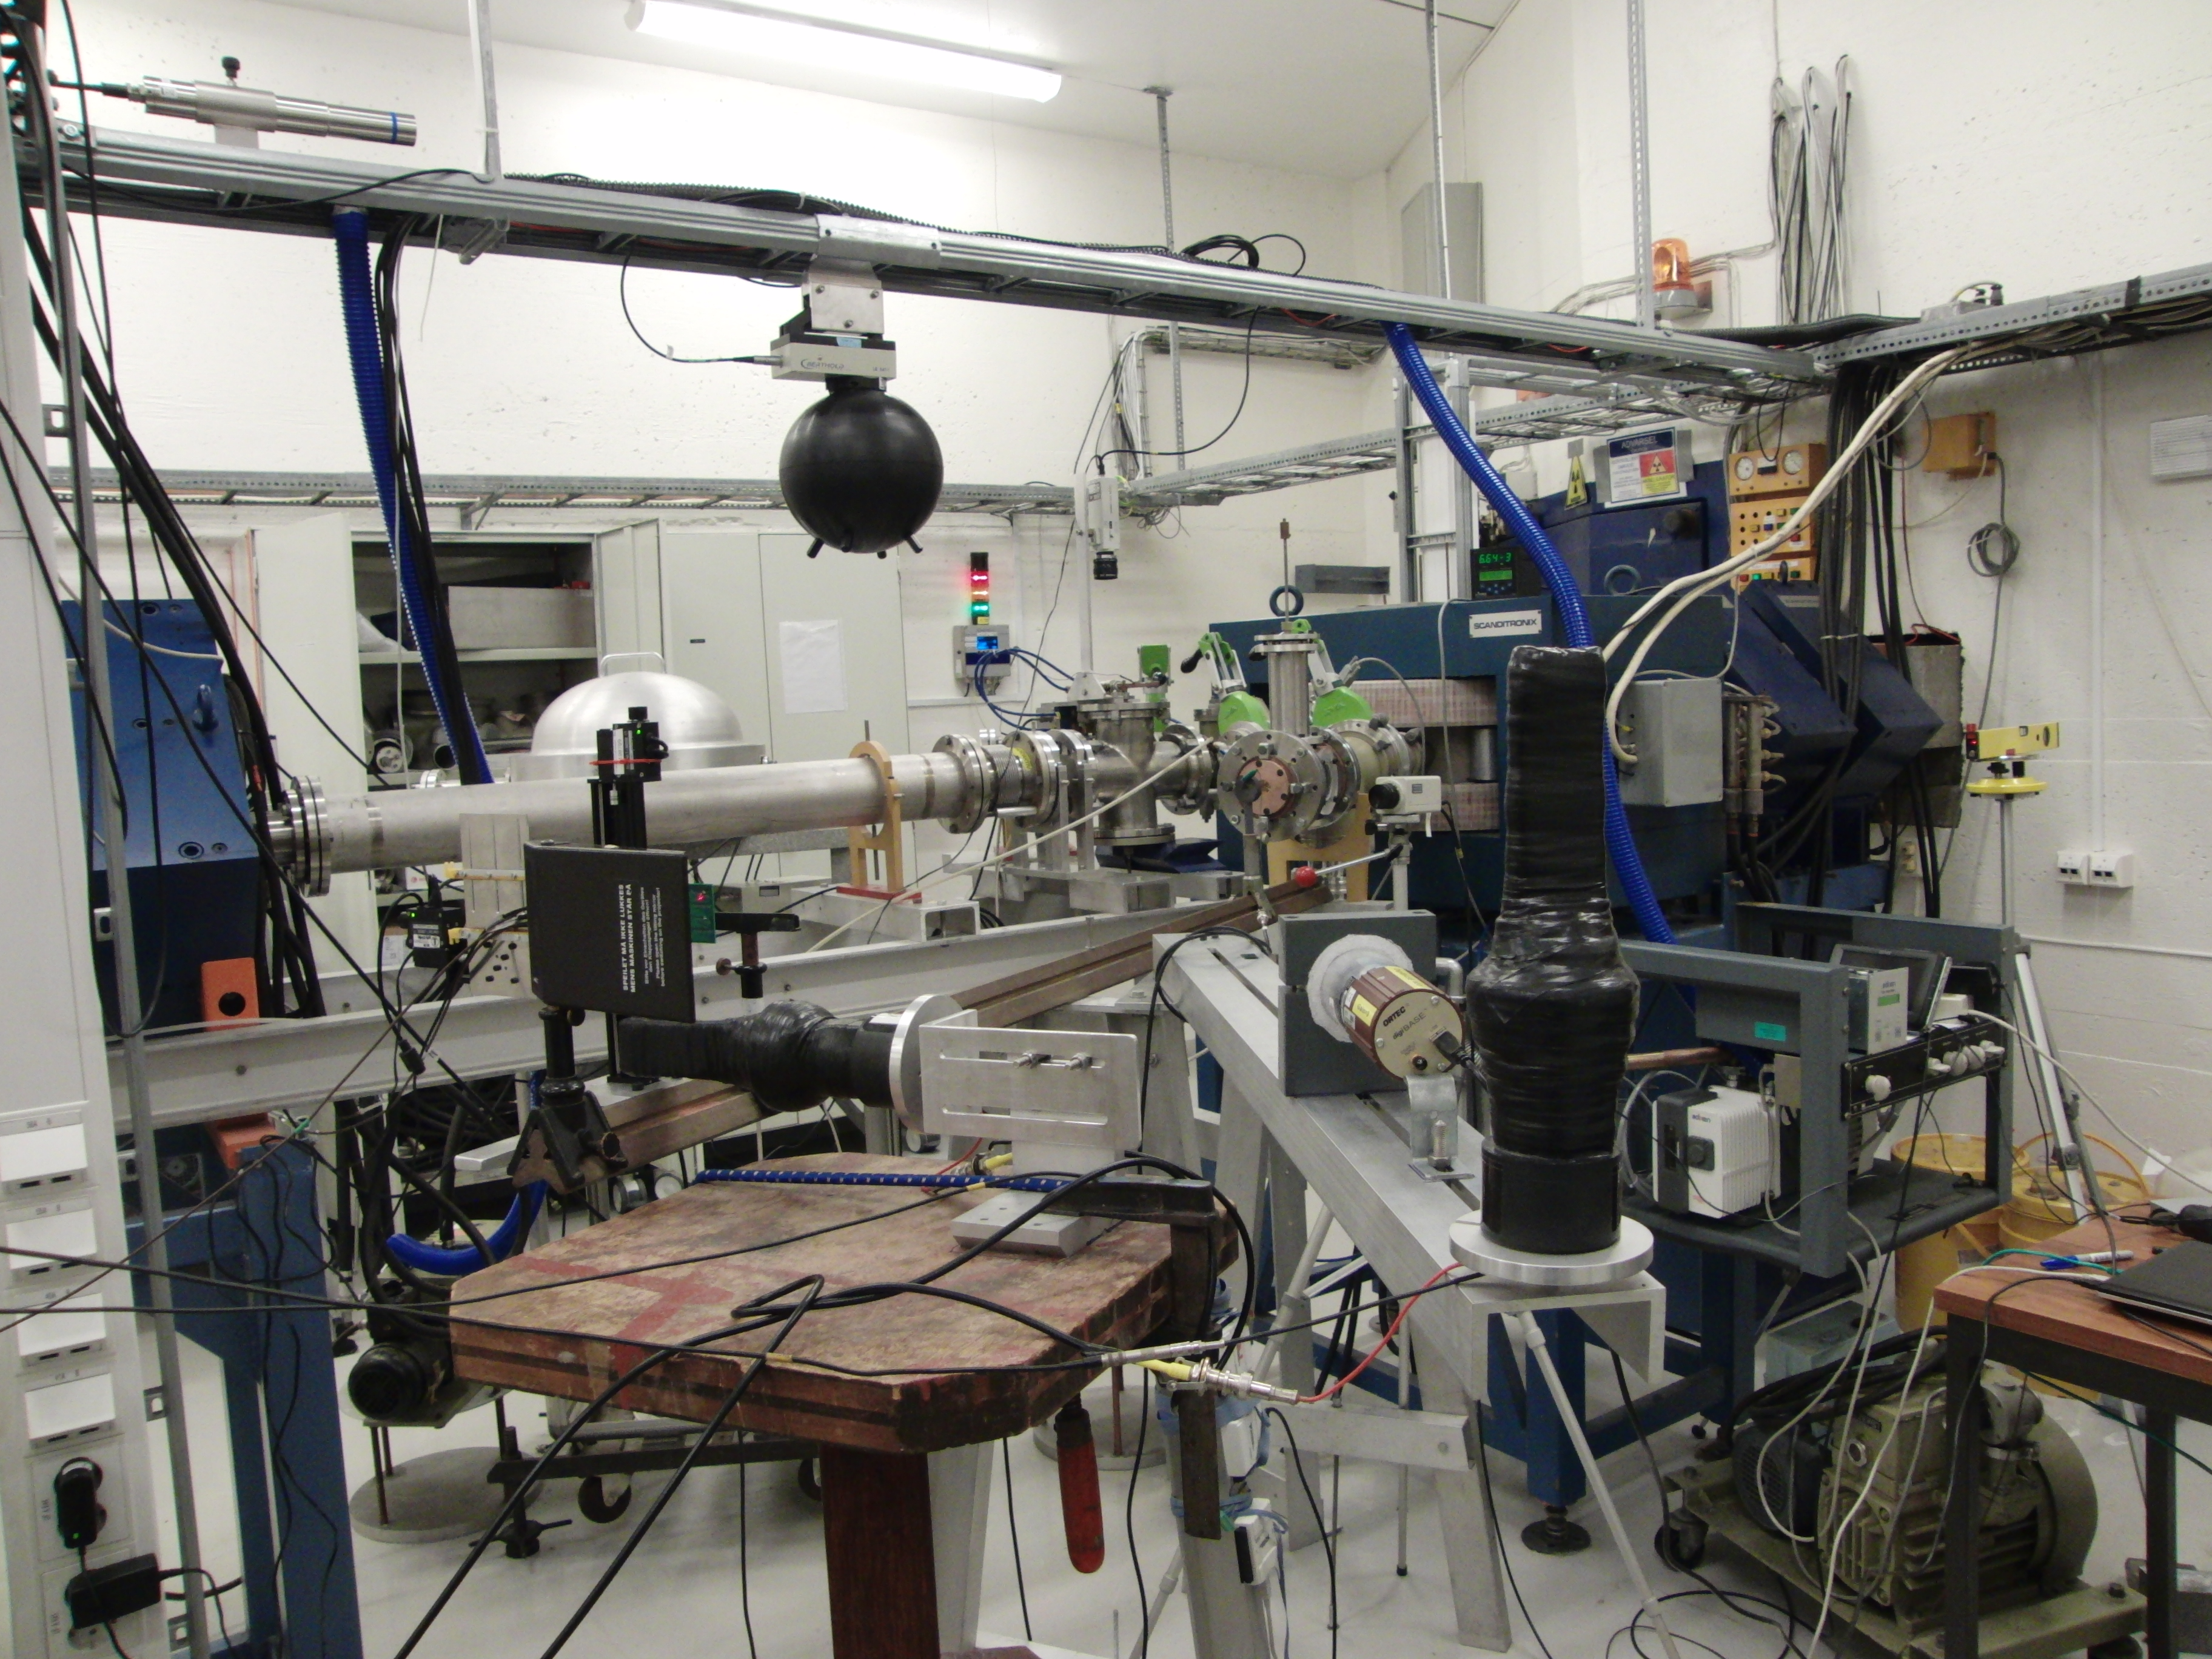
\includegraphics[width=\textwidth]{experiment_area.jpg}
  \caption{Picture of the experimental area}
  \label{experiment_area}
\end{figure}


\newpage
\begin{table}[!htbp]
 \centering
\begin{tabular}{|l|p{10cm}|}\hline
Equipment & Explanation  \\ \hline \hline
Scintillator & A plastic scintillator with photomultiplier. Was used to measure relative radiation. We had two of these, one that was placed right under \acf{DUT} and one that was placed 75cm away from \ac{DUT}. We only used the one 75cm away during the experiment.   \\ \hline
High voltage regulator & Voltage for the photomultiplier. 800V was used  \\ \hline
8 test boards &  TPS51200, MIC69302WU, SN74AVCB16245, SN74AVC2T245, QS3VH257, SY89831U, ADN2814 and MAX3748 \\ \hline 
SRAM-board  & A PCB board with 4 \ac{SRAM} cells that was used to characterise the beam and to measure scintillator counts \\ \hline
SF2 starter kit & A starter kit board with the Smart Fusion 2(SF2) chip.  \\ \hline
Computer  & A VPN connection was set on a computer inside the experimental hall, so that we were able to control the experiment from the control room. The computer was running LabView to control the experiment. Data was also saved on the computer\\ \hline
USB DAQ  & Data acquisition board form National Instruments(NI). Used to establish analog and digital connection to the test boards and send data to the computer. \\ \hline
Radiation film  & A film that reacts when radiated with protons. Used to identify the beam. \\ \hline
Counting controller  & A device that counts either rising or falling edges of a signal. \\ \hline
leveled laser  & This was used to pinpoint the center of the beam.\\ \hline
Mirror & Used to reflect the laser beam to the backside of the test boards.\\ \hline
XY-controller  & Connected to the computer so we can change the position of the test boards from outside the experimental area\\ \hline
\end{tabular}
\caption{Equipment used in the experiment}
\label{equipment}
\end{table}

\subsection{Measurement equipment and test boards}
\subsubsection{\ac{SRAM} board}
A \ac{SRAM} memory chip is very sensitive to \acf{SEE}, and can be used to measure relative radiation by constantly checking for \ac{SEU}.

The method of detecting an Single Event Upset (SEU) in a \ac{SRAM} is rather straight
forward, as can be seen in the flow diagram of figure \ref{flowchart}. There is an initial startup
phase where a known pattern is written to all the addresses in the \ac{SRAM}. When
the startup phase is done, the value from the first address is read back and compared
to a known value by XORing the known value with the one read. If they are not equal a SEU has occurred,
and a the XOR-function will go high and a 1 will be added to a SEU counter.
The correct value is then written back to the address and the system moves on to the next address.
  
A checkerboard pattern, a pattern of alternating ones and zeros, is used when writing
to the \ac{SRAM}. To check for stuck bits, the bit pattern in the whole address space is inverted after each read. 

From earlier experiment with the \ac{SRAM} chip, the cross section(the probability that an incoming particle will induce an SEU) is a known, and is found to be to be $\unit{1.14\e{-6}}{\centi\square\meter}$.
By counting number of SEU during an experiment, we can by dividing on the cross section find how many particles that hits the chip.
The \ac{SRAM} board that we used consist of 4 \ac{SRAM} chips, a flash based \ac{FPGA}, connections and supporting electronics.
The \ac{FPGA} on the \ac{SRAM} PCB is designed with RS485 two-way communication which makes it possible to edit firmware as well as sending data out. 
Through the experiment the \ac{SRAM} PCB was connected with RS485 to Opal Kelly XEM3001 which gave us connection to a computer. On the computer we ran a LabVIEW program, that made us able to monitor data, as well as doing some settings. 
The \ac{SRAM} board also had an optical input for scintillator counts, so we could by the use of this board also monitor scintillator counts.

\begin{figure}[!htbp]
  \centering
  \includegraphics[height=8cm, width=4cm]{SRAM_flowchart.png}
  \caption{Flowchart for SEU detection}
  \label{flowchart}
\end{figure}

In figure \ref{labview_SRAM} bellow you can see how the labVIEW program looked like. From here we can monitor SEU on all the 4 \ac{SRAM} cells, and see scintillator counts, reset counters, see time from start as well as other things. \ac{SRAM}1-10 as you can see on the left side, is different \ac{SRAM}-board.

\begin{figure}[!htbp]
  \centering
  \includegraphics[width=\textwidth]{SRAM_labview.png}
  \caption{LabVIEW program for the \ac{SRAM}}
  \label{labview_SRAM}
\end{figure}

\FloatBarrier

\subsubsection{Scintillator counter}
A scintillator is a material that gives out light when it is exposed to ionised radiation. 
But a scintillator can't be used alone, other than to see that there are radiation.
To get a more accurate measurement, we will need a \acf{PM-tube}. The PM-tube concerts light pulses to current by an electron avalanche process. This process is very sensitive to radiation.\cite{rad_phys}
The pulses could be measured with the SRAM board or a counter of some kind, we used the SRAM board during the experiment.

\newpage

\subsubsection{X-Y-positioning system}
The X-Y-positioning system is a system that makes it possible to mount our PCBs and move them in X and Y direction. This could be controlled directly on the X-Y-system or through a labVIEW program on the computer.
This was used when doing the beam profile as discussed in chapter \ref{beam_setup}, to be able to do changes on the position from the control room. In figure \ref{xy-table} you can see how the labVIEW program and picture of the X-Y-positioning system.

\begin{figure}[!htbp]
\centering
  \begin{subfigure}{.45\textwidth}
  \centering
  \includegraphics[width=\linewidth]{XY_front.jpg}
  \caption{SN74AVC2T245 board1}
  \end{subfigure}
  \begin{subfigure}{.45\textwidth}
  \centering
  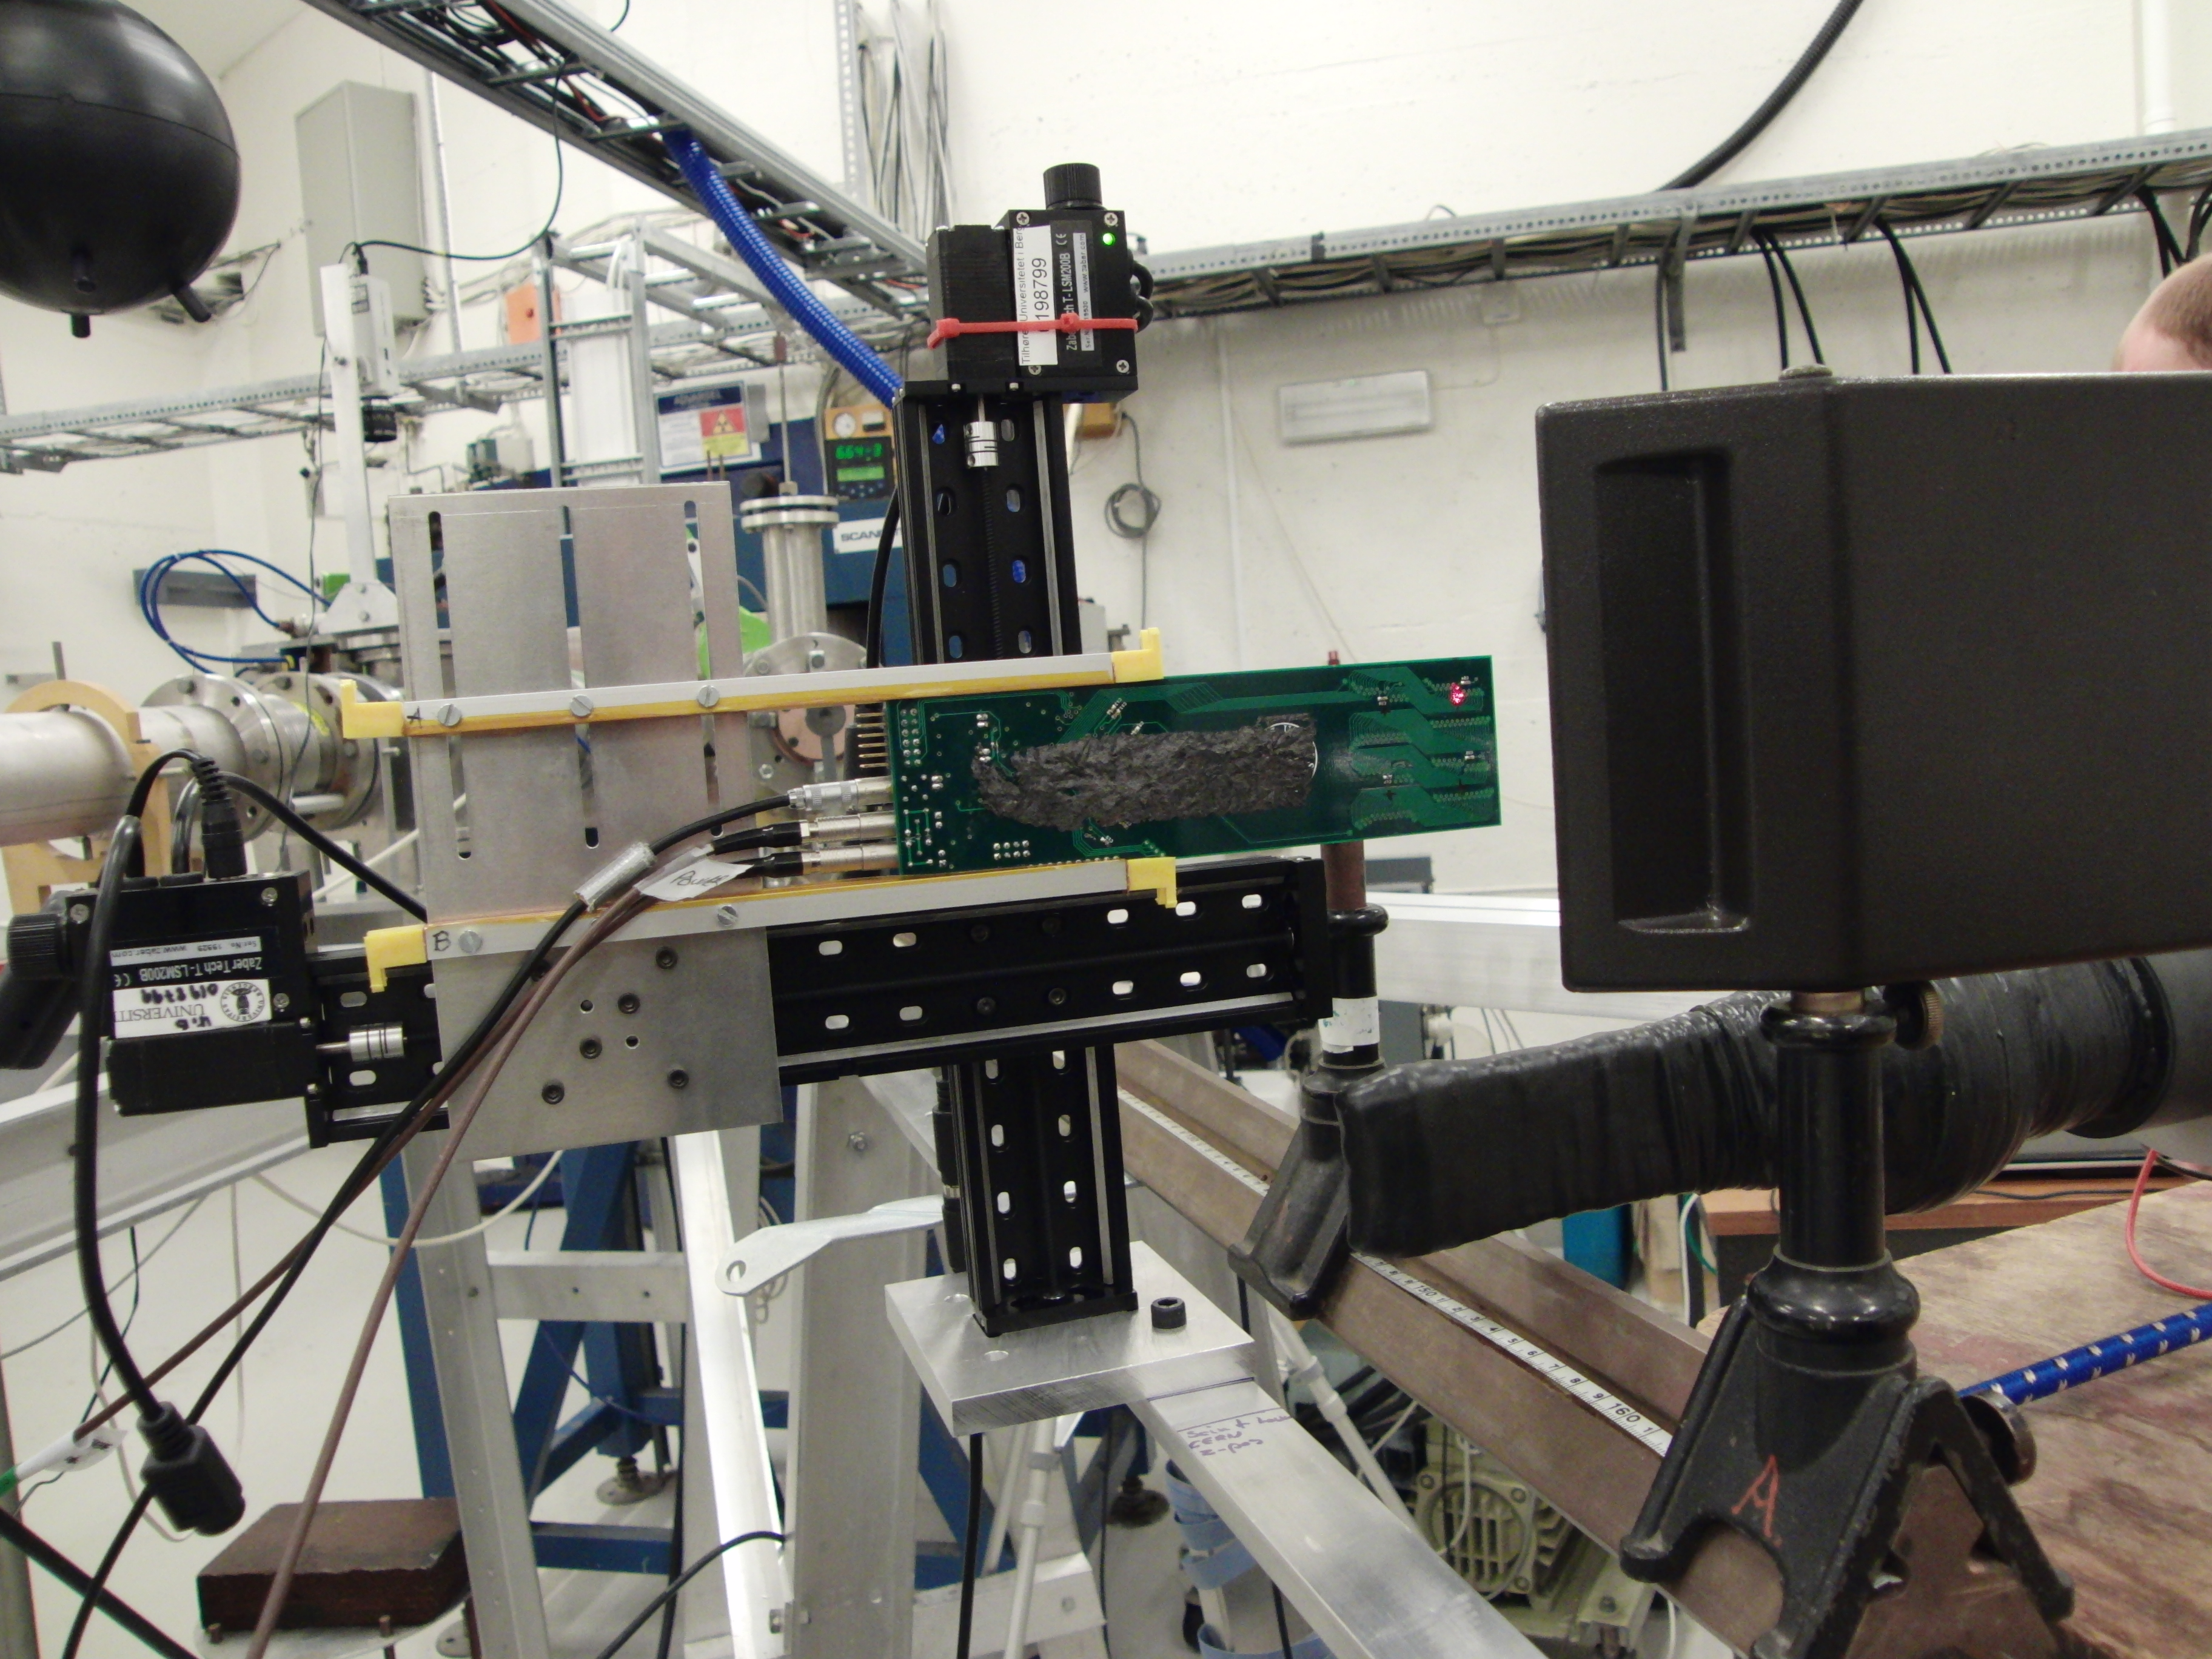
\includegraphics[width=\linewidth]{XY_back.jpg}
  \caption{SN74AVC2T245 board2}
  \end{subfigure}
 \caption{X-Y-positioning system upfront and behind, with SRAM-board mounted}
 \label{xy-table}
\end{figure}
\newpage

\subsection{Preparation and characterization of the beam}
Before we could start testing of the boards, the cyclotron had to be made ready for a proton beam and the magnet controlling the direction had to be put in the right position to get the beam out in experiment area 2.

\subsubsection{Purpose of tests}
The purpose of testing these board is to see if they are able to survive in a radiated area, as we will find at the \ac{LHC}, see section \ref{how_to_test}.
To make sure that we know the limit of the \ac{IC}s, the \ac{IC}s was radiate until a error occurred, current consumption drastically increased or the \ac{IC} received a much higher dose than was required without error.
Every IC that has been tested, are ICs that are going to be used in creation of the new RCU2 board.

\subsubsection{Beam setup}
  \label{beam_setup}
When the beam was set, we could start the characterization of the beam.
The first thing to do is to get an understanding of the beam,
too see that it hits around the area that we expect at our test position 125$\centi\meter$ from beam exit.
This was done by using radiation films that turns black when exposed to radiation. 
One of these was put right in front of the beam exit and one in front of \acf{DUT}-area to see how the beam looks like at the two positions.
This gave us a rough center position. A more precise calibration was done by the use of the \ac{SRAM} board and the scintillator. 
By measuring the relation between scintillator counts on the scintillator which was in a locked position and SEU on the \ac{SRAM} that was connected to a XY-position system(which made the \ac{SRAM} freely to move), we were able to find a more precise position of the beam center by seeing which position gave us highest SEU counts compared to scintillator counts.

This had to be done every day at startup, before we could start the actual tests.
When the beam center is found and everything works as it should, the laser was placed in a position so that the laser beam points to where we had found center of the beam to be. After that we could replace the \ac{SRAM} board with the PCB that we were going to test.
We were able to control the intensity(Current) of the beam freely from the control room inside the limitation of the beam (for protons that is up to 100 $\micro\ampere$), but we kept us in the area between 100 $\pico\ampere$ to a few $\nano\ampere$. This way the radiation dose to the test boards can be controlled. The beam intensity could be measured by putting a Faraday Cup(FC) in front of the beam. But the FC had to be removed when tests were running, since it will block the beam.

We were running 3 labVIEW programs at all time through the experiment, one for controlling the XY-position system,
one for the \ac{SRAM} board(to measure SEU and scintillator counts when calibrating and to get scintillator counts during the tests) and one program for each of the test boards.
The \ac{SRAM} and test board programs were constantly saving data on the disk.

\newpage

\section{Results and calculations from beam test at OCL}
The radiation was done in 5 days divided in two periods 13.11-15.11 and 28.11-29.11. I had made two version of most of the boards, the exception is ADN2814 and MAX3748 which I only made one version of.
The boards that where tested the first time are: $TPS51200_1, MIC69302WU_1, SN74AVCB16245_1, SN74AVC2T245_1,$
$QS3VH257_1$ and $SY89831U_1$ tested in that order. The first time at OCL we were given an beam of 28MeV, but the second time the lab personnel manage only to produce a beam of 25MeV.
When the beam gets out through the beam exit the energy will be reduced by crashing with air particles(~21keV per cm), so at DUT area the beam was approx ~25MeV and ~22MeV.

The result is presented after type, so that the two boards of the same type is presented together. 

\subsection{Calibration process}
As explained in chapter $\ref{beam_setup}$, we had to start with finding the center of the beam. In table $\ref{test_15.11}$ you can see the results from our calibration 15.11.2013. You can see that position x = -2,5 and y = -1 gives highest relation between SEU on the \ac{SRAM} and scintillator counts. A total of 4 tests in that position was done and the average value gives us 0,0948.
This value was used to calculate from scintillator counts to SEU. cross section(the probability that an incoming particle will induce an SEU) is known for the \ac{SRAM} board. The CS is given in equation \ref{CS}.

% Table generated by Excel2LaTeX from sheet 'Sheet1'
\begin{table}[!htbp]
  \centering
    \begin{tabular}{|r|r|r|r|r|r|}\hline
    Calibration test nr.: & x     & y     & Scint rel & SEU(\ac{SRAM}) & SEU(\ac{SRAM})/sc \\ \hline \hline
    1     & -0,8  & -1    & 27798 & 1463  & 5,26E-02 \\ \hline
    2     & -1,3  & -1    & 17721 & 1239  & 6,99E-02 \\ \hline
    3     & -1,8  & -1    & 12904 & 1203  & 9,32E-02 \\ \hline
    4     & -2,3  & -1    & 13361 & 1276  & 9,55E-02 \\ \hline
    5     & -2,8  & -1    & 12786 & 1238  & 9,68E-02 \\ \hline
    6     & -3,3  & -1    & 12342 & 1156  & 9,37E-02 \\ \hline
    7     & -2,5  & -1    & 11696 & 1223  & 1,05E-01 \\ \hline
    8     & -2,5  & -1,5  & 11027 & 1075  & 9,75E-02 \\ \hline
    9     & -2,5  & -2    & 11835 & 1063  & 8,98E-02 \\ \hline
    10    & -2,5  & -0,5  & 15593 & 1540  & 9,88E-02 \\ \hline
    11    & -2,5  & 0     & 12620 & 1034  & 8,19E-02 \\ \hline
    12    & -2,5  & -1    & 65280 & 5999  & 9,19E-02 \\ \hline
    13    & -2,5  & -1    & 52752 & 4803  & 9,10E-02 \\ \hline
    14    & -2,5  & -1    & 57229 & 5250  & 9,17E-02 \\ \hline
    \end{tabular}%
      \caption{Calibration tests 15.11.2013}
  \label{test_15.11}%
\end{table}%

\begin{equation}
scint\_conv = \frac{SEU(\ac{SRAM})} {scintillator counts} = 0,0948
\label{scint_conv}
\end{equation}

\begin{equation}
CS = 1,14e-6
\label{CS}
\end{equation}

\subsection{Test results}
The tests was controlled and monitored through a LabVIEW program for each of the different IC. When testing ADN2814 and MAX3748 there was also needed a SF2 board, to configure and monitor the input signal. A complete result of the tests can be found in appendix \ref{appendix}.
The point of this test was to see that these ICs would survive in a radiated area. The total dose of 10 years in ALICE-experiment is estimated to be a few kRad. If a IC survives more than 10 times that, we can be quite sure that it will survive the radiation it will receive at CERN.
In table \ref{dose_15.11} and \ref{dose_28.11} you can see how long each ICs has been exposed too radiation, the dose they has been received and if an error occurred.

\begin{table}[!htbp]
 \centering
\begin{tabular}{|l|l|l|l|}\hline
Device & Exposed time[s] & Dose[Rad] & Error \\ \hline \hline
$TPS51200$ & 2065 & 41800 & No \\ \hline
$MIC69302WU_1$ & 2240 & 164000 & No \\ \hline
$SN74AVCB16245_1$ & 967  & 65200 & No \\ \hline
$SN74AVC2T245_1$ & 860  & 4600 & Yes \\ \hline
$QS3VH257_1$ & 795  & 52800 & No \\ \hline
$SY89831_1$ & 1251 & 93500 & No \\ \hline
\end{tabular}
\caption{Tests at OCL 15.nov 2013}
\label{dose_15.11}
\end{table}

\begin{table}[!htbp]
 \centering
\begin{tabular}{|l|l|l|l|}\hline
Device & Exposed time[s] & Dose[Rad] &  \\ \hline \hline
$ADN2814/_run1$ & 1273 & 20200 & Yes \\ \hline
$ADN2814/_run2$ & 2286 & 324900 & Yes \\ \hline
$MAX3748$ & 2384 & 442200 & No \\ \hline
$TPS51200_2$ & -\textsuperscript{*} & -* & -* \\ \hline
$MIC69302WU_2$ & 1385 & 383800 & No \\ \hline
$SN74AVCB16245_2$ & 526  & 201400 & No \\ \hline
$SN74AVC2T245_2$ & 478  & 161600 & No \\ \hline
$QS3VH257_2$ & 264  & 110300 & No \\ \hline
$SY89831U_2$ & 921  & 165800 & No \\ \hline
\multicolumn{4}{l}{\textsuperscript{*}\footnotesize{The board wouldn't work at test time}}
\end{tabular}
\caption{Tests at OCL 27-28.nov 2013}
\label{dose_28.11}
\end{table}

\begin{figure}[!htbp]
  \centering
  \includegraphics[width=\textwidth]{flux_all_test1.jpg}
  \caption{flux for each component radiated 15.11.2013}
  \label{flux_all1}
\end{figure}

\begin{figure}[!htbp]
  \centering
  \includegraphics[width=\textwidth]{Flux_vs_time_all.jpg}
  \caption{flux for each component radiated 15.11.2013}
  \label{flux_all2}
\end{figure}
\newpage
In figure $\ref{flux_all1}$ and $\ref{flux_all2}$ you can see graphs of flux vs time for the different test boards. The reason the graphs don't go as linear as one would expect, is that the beam sometimes stopped and had to restarted, and that we increased the intensities when we wanted things to go faster.
\FloatBarrier

\subsubsection{TPS51200}
This was the first board that was tested. To measure the current going into the board, we added a 220$\ohm$ resistor on the input, and measured over this resistor to calculate the current.
A 3v3 voltage was supplied from the DAQs analog outputs. The output voltage was also monitored, through a analog input on the DAQ-box.
The intensity was a little low on this test. To make the testing process faster the intensity was increased during the later experiments.

The IC worked after a dose of 40kRad, but we could see a little increase in current after a dose of 25kRad. The output voltage is close to stable, a few mV up and down, but not noteworthy.
Two PCBs of this type was tested, but only one worked when we was at OCL to do the testing.

\begin{figure}[!htbp]
  \includegraphics[width=.45\textwidth]{current_voltage_tps.jpg}
  \caption{TPS51200 - Current/Voltage vs Dose}
  \label{TPS51200_1}
\end{figure}

\FloatBarrier

\subsubsection{MIC69302WU}
The first board was tested 15.11.13 and the second board was tested 28.11.13. During the test of the first board we increased the intensity of the beam quite allot, that can be seen from the flux graph, figure \ref{flux_all1}.
The current was measured, by adding a 220$\ohm$ resistor on the input, and measured the voltage over this resistor to calculate the current. 

This IC had an unexpected reaction to radiation. You can see from both of the graphs that the current is decreasing and voltage is increasing, normally we would expect the opposite, or at least that the current would increase.
As seen from the graph in figure \ref{MIC69302WU_both} it starts quite early to decrease in current, but as you can see it also stabilize after a while. The output voltage is mostly stable, there were a increase of ~2\% on both the tests.

\begin{figure}[!htbp]
\centering
  \begin{subfigure}{.45\textwidth}
  \centering
  \includegraphics[width=\linewidth]{current_voltage_mic.jpg}
  \caption{MIC69302WU board1}
  \label{MIC69302WU_1}
  \end{subfigure}
  \begin{subfigure}{.45\textwidth}
  \centering
  \includegraphics[width=\linewidth]{current_volt_dose_MIC.jpg}
  \caption{MIC69302WU board2}
  \label{MIC69302WU_2}
  \end{subfigure}
 \caption{MIC69302WU - Current/Voltage vs Dose}
 \label{MIC69302WU_both}
\end{figure}

\FloatBarrier

\subsubsection{SN74AVCB16245}
The current was measured in the same way as the two previously circuits, a 220$\ohm$ resistor was placed in series with power supply, and voltage over the resistor was measured and used to calculate current. To make sure that the circuit didn't drag current through the input on the chip we used a pMOS transistor, that was connected to supply pin on Drain, to ground on Source and Gate to a digital output from the DAQ. That way the current has to come from the power supply input, and not from the digital output of the DAQ. The outputs was measured by digital inputs on the DAQ.

It can be seen that the characteristics on the two test board are different, the reason for this is maybe because of different output load. The reason for the ``jumps`` in current is because the output is constantly changing from on to off, with a gap of 4 seconds.
This chips is not effected by radiation before a dose of approx 40kRad. That is more than enough for the purposes we are going to use this for.

\begin{figure}[!htbp]
\centering
  \begin{subfigure}{.45\textwidth}
  \centering
  \includegraphics[width=\linewidth]{current_4245.jpg}
  \caption{SN74AVCB16245 board1}
  \label{SN74AVCB16245_1}
  \end{subfigure}
  \begin{subfigure}{.45\textwidth}
  \centering
  \includegraphics[width=\linewidth]{current_dose_42452.jpg}
  \caption{SN74AVCB16245 board2}
  \label{SN74AVCB16245_2}
  \end{subfigure}
 \caption{SN74AVC2T245 - Current vs Dose}
\end{figure}

\FloatBarrier

\subsubsection{SN74AVC2T245}
This chip is almost the same as the SN74AVCB16245. A 220$\ohm$ resistor was used at the input to measure current, a digital output from the DAQ was used to put the input high and low, and digital inputs was used to measure the outputs.

Something went wrong on the first test. After 740s and a dose of 98Rad the chips output was stuck at 1. The reason for this is unknown, I fear that this might be defected before we started the test, since it gives a totally different characteristics than test board nr2.
The input was switching from high to low every 4 second. If we look at the test results from board 2. the current goes unchanged up to 40kRad, and that is more than enough.
%her m� eg sjekke board1 etter eg har f�tt den tilbake, og se om den faktisk fungere. Kan hende at denne har v�rt �delagt f�r vi begynte.

\begin{figure}[!htbp]
\centering
  \begin{subfigure}{.45\textwidth}
  \centering
  \includegraphics[width=\linewidth]{current_t245.jpg}
  \caption{SN74AVC2T245 board1}
  \label{SN74AVC2T245_1}
  \end{subfigure}
  \begin{subfigure}{.45\textwidth}
  \centering
  \includegraphics[width=\linewidth]{current_dose_t2452.jpg}
  \caption{SN74AVC2T245 board2}
  \label{SN74AVC2T245_2}
  \end{subfigure}
 \caption{SN74AVC2T245 - Current vs Dose}
\end{figure}

\FloatBarrier

\subsubsection{QS3VH257}
This was also tested by putting a 220$\ohm$ resistor in series with the power supply, in the same way as the others. For the Select input a analog output signal from the DAQ was used. The input signals was set by digital outputs from the DAQ. The outputs was measured by digital inputs on the DAQ.
The select input was changed every 4 second and the inputs was changed every 18second.

Both of the boards worked fine through the tests. 
We see that we have small increase in current before 30kRad, after that it increases quite allot. We couldn't see any errors on the output during the experiment, but it should probably not be exposed to more than 30kRad.

\begin{figure}[!htbp]
\centering
  \begin{subfigure}{.45\textwidth}
  \centering
  \includegraphics[width=\linewidth]{current_q.jpg}
  \caption{QS3VH257 board1}
  \label{QS3VH257_1}
  \end{subfigure}
  \begin{subfigure}{.45\textwidth}
  \centering
  \includegraphics[width=\linewidth]{current_dose_q2.jpg}
  \caption{QS3VH257 board2}
  \label{QS3VH257_2}
  \end{subfigure}
 \caption{QS3VH257 - Current vs Dose}
\end{figure}

\FloatBarrier

\subsubsection{SY89831}
This is a buffer used to make 1 clock to 4 clocks. This chip required a high current to work, and since the labVIEW DAQ box only delivers 5mA on the analog outputs, I had to use the 5V output on the DAQ that could deliver up to 200mA. But I also needed to have a 3v3 power supply, this was solved by using a modified MIC69302WU board, so that it delivers 3.3V and can be used to supply this IC. To measure the current, I had to use 20$\ohm$ resistor to make sure that I didn't had a voltage drop, because of the high current consumption. voltage over this resistor was measured to get current.
To test that the chip worked as it should, two analog outputs from the DAQ was used to make a DC differential input. This was measured by digital inputs on a DAQ to see that i goes high and low according to the input.

A difference in characteristics can also be seen here. This may be because two different footprint for the PCB was used, and therefore some difference can be seen. We see a small increase in current on both of the boards, but not noteworthy, compared to how much current this IC is using.


\begin{figure}[!htbp]
\centering
  \begin{subfigure}{.45\textwidth}
  \centering
  \includegraphics[width=\linewidth]{current_sy.jpg}
  \caption{SY89831 board1}
  \label{SY89831_1}
  \end{subfigure}
  \begin{subfigure}{.45\textwidth}
  \centering
  \includegraphics[width=\linewidth]{current_dose_SY2.jpg}
  \caption{SY89831 board2}
  \label{SY89831_2}
  \end{subfigure}
 \caption{SY89831 - Current vs Dose}
\end{figure}

\FloatBarrier

\subsubsection{ADN2814}
This IC is a little special and was hard to get a good test on. This is a clock and data return circuit, with a limiting amplifier.
The SF2 board was used to code a clock and data into a differential Manchester signal, that was sent into the IC. Out of the IC we get a clock and a limited Manchester coded data signal. The Mancheseter coded data signal was decoded on the Igloo FPGA on SF2 board, so that we get out a clock and data. The data was tested by delaying the original data through a few D-latches, so that the original and returned data was close to alike. Then we could compare the original data with the one from the chip through a XOR-function, to see if they was alike. This function was triggered by a 80Mhz clock from the SF2 board. If they aren't alike when the clock rises, a 1 was added to a counter. The value of the counter was constantly sent through the UART of the SF2 board.

The way the clock was tested was a little harder process since the clock was so fast (160Mhz).
This was solved, was by adding a third clock with the same frequency (160Mhz) that was $90\,^{\circ}$ of from the two others, when this goes high I called on the XOR-function, to see if the two other clocks are the same. if they are alike, nothing happens, if they are not the program adds 1 to a counter, which constantly writes its current value to a UART.
The problem here is that for each time the SF2 board was programed the clock was slightly different, that made either the clock out of sync or the data out of sync, so that the code didn't work as it should.
This circuit also requires allot of current, therefore the same solution as for SY89831 was used, using MIC69302WU as a power supply and measure the current on that PCB.

The current didn't change before a dose of 200kRad had been received, but we got a clock error at a dose of ~11kRad, and a data error after a dose of ~8kRad.
How good this test really is, could be discussed, since we don't have any data on the clock and data, other than that the XOR-function failed. What really failed, and how much is impossible to know. It could be a slightly delay on a clock or the data, or maybe the clock just disappeared for a moment. There could also be a problem with the clocks on the SF2 board.

\begin{figure}[!htbp]
\centering
  \begin{subfigure}{.45\textwidth}
  \centering
  \includegraphics[width=\linewidth]{current_dose_ADN_t1.jpg}
  \caption{ADN2814 test1}
  \label{ADN2814_1}
  \end{subfigure}
  \begin{subfigure}{.45\textwidth}
  \centering
  \includegraphics[width=\linewidth]{current_dose_ADN_t2.jpg}
  \caption{ADN2814 test2}
  \label{ADN2814_2}
  \end{subfigure}
 \caption{ADN2814 - Current vs Dose}
\end{figure}

\begin{figure}[!htbp]
\centering
  \begin{subfigure}{.45\textwidth}
  \centering
  \includegraphics[width=\linewidth]{error_dose_ADN_t1.jpg}
  \caption{ADN2814 test1}
  \label{ADN2814_1e}
  \end{subfigure}
  \begin{subfigure}{.45\textwidth}
  \centering
  \includegraphics[width=\linewidth]{error_dose_ADN_t2.jpg}
  \caption{ADN2814 test2}
  \label{ADN2814_2e}
  \end{subfigure}
 \caption{ADN2814 - Relative errors vs Dose}
\end{figure}

\FloatBarrier

\subsubsection{MAX3748}
This circuit has the same purpose as ADN2814, the difference is that this one only return the limited Manchester coded signal, and no clock. The process for testing the data is the same as for the ADN2814.
The decoding process return clock and data, but since they are related to another, a error on the clock would mean an error at the data. So by measuring data, we can be sure that there are no clock errors as well. 

After a dose of over 400kRad this chip still worked, and current consumption was stable through the hole radiation process.

\begin{figure}[!htbp]
\centering
  \begin{subfigure}{.45\textwidth}
  \centering
  \includegraphics[width=\linewidth]{current_dose_MAX.jpg}
  \caption{Current vs Dose}
  \label{MAX3748}
  \end{subfigure}
  \begin{subfigure}{.45\textwidth}
  \centering
  \includegraphics[width=\linewidth]{error_dose_MAX.jpg}
  \caption{Errors vs Dose}
  \label{MAX3748_error}
  \end{subfigure}
 \caption{MAX3748}
\end{figure}

\FloatBarrier

\newpage

\subsection{Calculation of dose}
After a radiation test on one of the PCB, we knew the exposed time and scintillator counts. From the calibration we knew the relation between scintillator counts and SEU on the \ac{SRAM}, and cross section(CS). 
We start by calculating SEU from the factor given in equation $\ref{scint_conv}$. Then we calculate the fluence at \ac{DUT} as seen in equation $\ref{FluenceDUT}$, and by this we can calculate the flux, see equation $\ref{flux}$.
To calculate the dose from here we need to know some more factors. We run a simulation on a program called FLUKA. This program is used to simulate particles in different environment. We simulated a proton beam of 28MeV and 25MeV in air, and inserted the distance from BE(Bean exit). The results can be seen in table $\ref{FLUKA_15}$.
Then we had enough information to calculate the dose. As seen from equation $\ref{FluenceBE}$ we are able to find the Fluence at BE. And from there we can calculate the dose at \ac{DUT}, see equation \ref{DoseDUT}.


% Table generated by Excel2LaTeX from sheet 'Fluka'
\begin{table}[!htbp]
  \centering
    \begin{tabular}{|l|l|} \hline
    Fluka simulation results 28MeV &  \\\hline\hline
    Dose/primary particle at DUT[Gy] & 4,08E-10 \\\hline
    Primary particles at Beam exit & 1 \\\hline
    Primary particles at DUT & 0,1331 \\\hline
    Beam intensity reduction  at DUT & 7,513148009 \\\hline
    \end{tabular}%
      \caption{FLUKA simulation with 28MeV proton beam}
  \label{FLUKA_15}%
\end{table}%


\begin{equation}
FluenceDUT = \frac{SEU}{CS}
\label{FluenceDUT}
\end{equation}

\begin{equation}
Flux = \frac{Fluence}{time}
\label{flux}
\end{equation}

\begin{equation}
FluenceBE = \frac{fluenceDUT}{primary_particlesDUT}
\label{FluenceBE}
\end{equation}

\begin{equation}
DoseDUT[Gy] = FluenceBE \times \frac{Dose}{primary particle at DUT}
\label{DoseDUT}
\end{equation}

\begin{equation}
1 Rad = 100 Gy
\label{Gy_to_Rad}
\end{equation}

\newpage
\subsection{Discussion of the result}
Most of the testing was done 15.nov and 28.nov. The other days was used to get familiar with the instruments and equipment that was being used, to prepare the setup and setting up the beam.
There are almost impossible to get the same beam two days at a row. Each day of testing is therefore different from each other. Since the testing was conducted in two periodes and a total of 4 test days, there are allot of uncertainties regarding the beam.
And that is also why we had to do calibration each day at start-up.

When we where going to measure the intensity at the BE, we placed a faraday cup in front of the beam, and connected it to a amperemeter on the kontroll panel, but since the current is so small, the measuring instrument will be affected by air currents, and there are also allot of uncertainties in the instruments. Therefore we only used the FC, to get a hunch of the actual intensity.

The are also some uncertainties regarding the DAQ box form NI. When measuring digital signal, we don't know if it goes from 0V to 3v3V as we would expect. Maybe in reality the low voltage is actually 0.4V and high voltage is actually 2.8V. If this is the case, it could be a problem with using this in our design.

As said before in \ref{beam_setup}, if a component survives 10 times more than what it will receive in a period of 10 years in ALICE, that is 0.6kRad, than it can be used in the design of RCU2.
Having that in mind, I would say that every component tested would have a green flag even though we had some errors when testing SN74AVC2T245 and ADN2814. Since the result after testing board two of SN74AVC2T245, was positive we can assume that something was wrong with the first board. When it comes to ADN2814, I would rather have time to test this even more, since the test done gave us so unclear results. But it manage to run error free until a dose of 8kRad, and that is more than enough for our use.
Some of the tests gave us some unclear results, and if we had more time and chances to use to lab it would have been nice to do some more testing.

\newpage

\section{Conclusion}


\newpage
\FloatBarrier

\section{Appendix}
\label{appendix}

\subsection{datasheets}
\label{datasheets}
% Table generated by Excel2LaTeX from sheet 'Sheet1'
\begin{table}
  \centering
    \begin{tabular}{|l|l|l|l|l|l|} \hline
    Calibration test nr.: & x     & y     & Scint rel & SEU(\ac{SRAM}) & SEU(\ac{SRAM})/sc \\ \hline \hline
    1     & 0     & 0     & 23813 & 1971  & 8,28E-02 \\ \hline
    2     & 0     & -0,5  & 37930 & 3867  & 1,02E-01 \\ \hline
    3     & 0     & -1    & 27527 & 2817  & 1,02E-01 \\ \hline
    4     & 0     & -1,5  & 34413 & 3360  & 9,76E-02 \\ \hline
    5     & 0     & -2    & 32713 & 2763  & 8,45E-02 \\ \hline
    6     & 0,5   & 0     & 38753 & 2709  & 6,99E-02 \\ \hline
    7     & -0,5  & 0     & 23420 & 2483  & 1,06E-01 \\ \hline
    8     & -1    & 0     & 20611 & 2232  & 1,08E-01 \\ \hline	
    9     & -1,5  & 0     & 21014 & 2410  & 1,15E-01 \\ \hline
    10    & -1,5  & 0     & 20676 & 2260  & 1,09E-01 \\ \hline
    11    & -2    & 0     & 35787 & 3776  & 1,06E-01 \\ \hline
    12    & -2,5  & 0     & 27847 & 2512  & 9,02E-02 \\ \hline
    \end{tabular}%
      \caption{Calibration tests 14.11.2013}
      \label{test_14.11}
\end{table}%

% Table generated by Excel2LaTeX from sheet 'Sheet1'
\begin{table}
  \centering
    \begin{tabular}{|l|l|l|l|l|l|}\hline
    Calibration test nr.: & x     & y     & Scint rel & SEU(\ac{SRAM}) & SEU(\ac{SRAM})/ sc \\ \hline \hline
    1     & -0,8  & -1    & 27798 & 1463  & 5,26E-02 \\ \hline
    2     & -1,3  & -1    & 17721 & 1239  & 6,99E-02 \\ \hline
    3     & -1,8  & -1    & 12904 & 1203  & 9,32E-02 \\ \hline
    4     & -2,3  & -1    & 13361 & 1276  & 9,55E-02 \\ \hline
    5     & -2,8  & -1    & 12786 & 1238  & 9,68E-02 \\ \hline
    6     & -3,3  & -1    & 12342 & 1156  & 9,37E-02 \\ \hline
    7     & -2,5  & -1    & 11696 & 1223  & 1,05E-01 \\ \hline
    8     & -2,5  & -1,5  & 11027 & 1075  & 9,75E-02 \\ \hline
    9     & -2,5  & -2    & 11835 & 1063  & 8,98E-02 \\ \hline
    10    & -2,5  & -0,5  & 15593 & 1540  & 9,88E-02 \\ \hline
    11    & -2,5  & 0     & 12620 & 1034  & 8,19E-02 \\ \hline
    12    & -2,5  & -1    & 65280 & 5999  & 9,19E-02 \\ \hline
    13    & -2,5  & -1    & 52752 & 4803  & 9,10E-02 \\ \hline
    14    & -2,5  & -1    & 57229 & 5250  & 9,17E-02 \\ \hline
    \end{tabular}%
      \caption{Calibration tests 15.11.2013}
\end{table}%

% Table generated by Excel2LaTeX from sheet 'Fluka'
\begin{table}
  \centering
    \begin{tabular}{|l|l|} \hline
    Fluka simulation results 28MeV &  \\\hline\hline
    Dose/primary particle at DUT[Gy] & 4,08E-10 \\\hline
    Primary particles at Beam exit & 1 \\\hline
    Primary particles at DUT & 0,1331 \\\hline
    Beam intensity reduction  at DUT & 7,513148009 \\\hline
    \end{tabular}%
      \caption{FLUKA simulation with 28MeV proton beam}
\end{table}%

% Table generated by Excel2LaTeX from sheet 'Fluka'
\begin{table}
  \centering
    \begin{tabular}{|l|l|}\hline
    Fluka simulation results 25MeV &  \\\hline\hline
    $\frac{Dose}{primary particle at DUT}$[Gy] & 2,94E-10 \\\hline
    Primary particles at Beam exit & 1 \\\hline
    Primary particles at DUT & 8,57E-02 \\\hline
    Beam intensity reduction  at DUT & 11,6713352 \\\hline
    \end{tabular}%
    \caption{FLUKA simulation with 25MeV proton beam}
  \label{FLUKA_28}%
\end{table}%


\FloatBarrier

\newpage
\bibliographystyle{plain}
\bibliography{Master_Thesis_Inge_Nikolai_Torsvik}
\end{document}